\section{Sanity check}
%%% TODO: Build bridge from previous chapter 
Having introduced our cell dynamics, we now want to take a look at the simulation results.
Therefore, we aim to compare our simulation results to results from an established cell model from~\cite{Bruna2012}. 
In~\cite{Bruna2012} the diffusion dynamics of first a point particle model and second a hard sphere model is studied. 
Thereby, the two density distributions:
\begin{itemize}
    \item the joint probability density function $P(\vec{X}, t)$ of the system of all cell centres $\vec{X}$ at time $t$,
    \item the marginal distribution function of the first particle $p(\vec{x}_1, t)$
\end{itemize}
play an important roll. \\
The joint probability density function $P(\vec{X}, t)$ is a function describing the positions of all particles in the system, while the marginal distribution function $p(\vec{x}_1, t)$ is a function describing only the position of the first particle. \\
It is sufficient to consider only the marginal distribution function of first particle, because all particle act similarly. \\ 
Gaining $p(\vec{x}_1, t)$ from $P(\vec{X}, t)$ is a big reduction of complexity, since we reduce from a high-dimensional PDE for $P$ to a low-dimensional PDE for $p$. 
The marginal distribution function the of first particle can always be determined via
\begin{center}
    $
    p(\vec{x}_1, t) = \int P(\vec{X}, t) \dequ \vec{x}_2 \dots  \dequ \vec{x}_{N_{BC}}.
    $
\end{center} 

\subsection{Reference simulations: Bruna and Chapman (2012)}
The most simple model that gets considered for the diffusion dynamics of cell systems is the point particle model. 
Here the cells get modeled with sizeless points that perform a Brownian motion on the domain. \\
Since the cells do not have a real size, no interaction between the cells can occur, since they will never hit upon each other.  

The paper~\cite{Bruna2012} analyses these dynamics on the domain 
\begin{center}
    $
    \Omega_{BC} = [-0.5, 0.5]^2,
    $
\end{center}
on which $N_{BC} = 400$ particles are located. \\
The movement of each point particle $\vec{x}_i$ in the simulation is given by the SDE
\begin{center}
    $\dequ \vec{x}_i(t) = \sqrt{2} \dequ B_t^{(i)}$, \hspace{0.5em} $1 \leq i \leq N_{BC}$,
\end{center}
which describes a Brownian motion in $\Omega_{BC}$.
The reflective boundary condition on $\partial \Omega_{BC}$ is imposed.
It is known, that the joint probability density of the particle system in this setup evolves according to the diffusion equation, i.e.
\begin{equation}
    \frac{\partial P}{\partial t}(\vec{X}, t) = \Delta_{\vec{X}} P = \nabla_{\vec{X}} \cdot [ \nabla_{\vec{X}} P]
    \label{eq:heat}
\end{equation}
inside of the domain. \\
Since all particles are independent, we can compute
\begin{equation}
    P(\vec{X}) = \prod_{i=1}^{N_{BC}} p(\vec{x}_i, t).
\end{equation}
Therefore, we obtain the marginal distribution function as 
\begin{align}
    \label{equ:marginalHeat}
    \frac{\partial p}{\partial t}(\vec{x}_1, t) = \Delta_{\vec{x}_1} p = \nabla_{\vec{x}_1} \cdot [ \nabla_{\vec{x}_1} p].
\end{align}

A next step that results in the hard sphere cell model (HSCM) is to give the cell particles a real size. \\
Let $0 < \epsilon \ll 1$ be the diameter of all cells that are now two dimensional discs with the same size. 
This changes the dynamics of the cells immense, since they now have chance to collide into each other which is a form of interaction. \\
The authors of~\cite{Bruna2012} also did a simulation with the HSCM. 
The setting is as similar as possible to the point particle model, because a main goal of the paper was to compare the diffusion characteristics of both models. 
There are still $N_{BC} = 400$ cells located on the domain. \\

The initial condition of both models follows a two dimensional normal distribution with the addition that the distance of each cell centre to all others is at least $\epsilon$.  
The used distribution $\mathcal{N}_2 \left( 
\scalebox{0.7}{$\begin{pmatrix} 0 \\ 0 \end{pmatrix}$}, 
\scalebox{0.7}{$\begin{pmatrix} 0.09^2 & 0 \\ 0 & 0.09^2 \end{pmatrix}$}
\right)$ has an integral of one over $\Omega_{BC}$. \\
We can compute this initial condition with Algorithm~\ref{alge:HSCMinitial}.
\begin{algorithm} \textbf{Computation of the initial cell system} \label{alge:HSCMinitial}
	\begin{enumerate} 
		\item Generate a point $\vec{x} \sim \mathcal{N}_2 \left( 
\scalebox{0.7}{$\begin{pmatrix} 0 \\ 0 \end{pmatrix}$}, 
\scalebox{0.7}{$\begin{pmatrix} 0.09^2 & 0 \\ 0 & 0.09^2 \end{pmatrix}$}
\right)$. 
		\item If for all already generated centres $\vec{x}_j: \norm[\vec{x} - \vec{x}_j] > \epsilon$ is true, use $\vec{x}$ as the next cell centre, otherwise discard the point and restart with step 1 until $N_{BC}$ cell centres are found. 
	\end{enumerate}	
\end{algorithm}

Since we do not want any overlap to occur during the whole simulation with the HSCM, the feasible domain for the whole cell system is not directly $\Omega_{BC}^{N_{BC}}$, but instead 
\begin{center}
    $\Omega_{BC}^{\epsilon} = \Omega_1^{\epsilon} \times \ldots \times \Omega_{N_{BC}}^{\epsilon}$, \\
    $\Omega_{i}^{\epsilon} = \Omega_{BC} \setminus ( \cup_{j \neq i} \mathrm{B}_{\epsilon}(\vec{x}_j))$, \hspace{0.5em} $1 \leq i \leq N_{BC}$,
\end{center}
where $\mathrm{B}_{\epsilon}(\vec{x}_j)$ denotes the ball around $\vec{x}_j$ with radius $\epsilon$. \\
This domain prevents overlaps between the cells by not allowing each cell to drift closer than $\epsilon$ to any other cell.  

HSCM cells perform the same Brownian motion as the point particles. \\
The next question is, how cell collisions are modelled. 
Unlike in our DCF model where cell interactions are modelled as forces acting inside of the domain, the cell collisions from the HSCM arise from the reflective boundary condition. \\
Let us assume that two cells $i$ and $j$ are given such that $\norm[\vec{x}_i - \vec{x}_j] = \epsilon$ is true. 
Then, both cell centres are located at the boundary $\partial \Omega_{BC}^{\epsilon}$. 
Here, the reflective boundary condition is still imposed and it causes both cells to bounce of from each other in the direction of the outward normal vector from the excluded area of the respectively other cell. \\ 

In~\cite{Bruna2012} the authors managed to compute the marginal distribution function of the first particle of the HSCM. 
In two dimensions it is given by:
\begin{equation}
    \frac{\partial p}{\partial t}(\vec{x}_1, t) = \nabla_{\vec{x}_1} \cdot \{\nabla_{\vec{x}_1}[p + \frac{\pi}{2}(N_{BC} - 1)\epsilon^2 p^2]\}.
    \label{eq:hard-sphere-p}
\end{equation}
We can see a connection to Equation~\ref{equ:marginalHeat}. 
Let us define a diffusion coefficient $$D_{\epsilon}(p) = 1 + \pi(N_{BC}-1)\epsilon^2p$$ that depends on the local partical density $p$ and the cell diameter $\epsilon$. 
For the point particles, we have $\epsilon = 0$ and $D_{\epsilon}(p) = 1$.
Thus, we can rewrite the first marginal to  
\begin{align*}
    \frac{\partial p}{\partial t}(\vec{x}_1, t) = \nabla_{\vec{x}_1} \cdot [D_{\epsilon}(p) \nabla_{\vec{x}_1} p]. 
\end{align*}
In the case of the hard spheres, where $\epsilon > 0$, we can compute
\begin{align*}
    \frac{\partial p}{\partial t}(\vec{x}_1, t) &= \nabla_{\vec{x}_1} \cdot [D_{\epsilon}(p) \nabla_{\vec{x}_1} p] \\  
    &= \nabla_{\vec{x}_1} \cdot [(1 + \pi(N_{BC}-1)\epsilon^2p) \nabla_{\vec{x}_1} p] \\
    &= \nabla_{\vec{x}_1} \cdot [\nabla_{\vec{x}_1} p + \pi(N_{BC}-1)\epsilon^2 p \nabla_{\vec{x}_1} p] \\
    &= \nabla_{\vec{x}_1} \cdot [\nabla_{\vec{x}_1} p + \pi(N_{BC}-1)\epsilon^2 \frac{1}{2}\nabla_{\vec{x}_1} p^2] \\
    &= \nabla_{\vec{x}_1} \cdot [\nabla_{\vec{x}_1} (p + \frac{\pi}{2}(N_{BC}-1)\epsilon^2 p^2)] \\
\end{align*}
to recover Equation~\ref{eq:hard-sphere-p}. \\ 
When considering \( D_\epsilon(p) = 1 + \pi(N_{BC}-1)\epsilon^2p \) to be the diffusion coefficient, we can conclude that an increase in the number of cells \( N_{BC} \), the cell diameter \( \epsilon \), or the local density \( p \) leads to an increased diffusion rate of the system.
Overall, we conclude that the bounce effect of the HSCM enhances the diffusion rate of the system's density.

Another evidence of this behavior is shown in Figure 2 in~\cite{Bruna2012}. \\
Here, we can see two Monte Carlo simulations. 
A Monte Carlo simulation is a computational technique that uses random sampling to model and analyse complex systems or processes that are difficult to solve analytically. 
It repeatedly generates random inputs according to specified probability distributions and computes the resulting outcomes to estimate quantities like averages, variances, or distributions. \\
In our case, the Monte Carlo simulations are used to track the positions of cell centres over time. 
Each simulation begins from an initial configuration of cells, which is consistently generated using Algorithm~\ref{alge:HSCMinitial}. 
After initialization, the prescribed dynamics - either the point particle model or the hard sphere model - are applied, and the positions of the cell centres are recorded at a fixed time point, $t=0.05$. \\
To visualise the results, we construct heatmaps representing the spatial distribution of cells at the final time. 
This is done by discretizing the domain into a uniform grid of sub squares. 
For each sub square, we count how many cells fall within it across all simulations. 
The resulting counts are normalised by dividing by the total number of cells $N_C$, the number of simulations, and the area of a sub square. This normalisation ensures that the heatmap represents a probability density, satisfying the mass conservation condition: \[\sum\limits_{i \: \in \text{ sub squares}} \text{value}_i \cdot \text{area}_i = 1. \]
This approach provides a smooth estimate of the empirical cell density, allowing direct comparison with the corresponding solutions of the diffusion equations.

Figure~\ref{fig:fig2BC12} shows the discussed graphic from~\cite{Bruna2012}. 
\begin{figure}
	\centering
    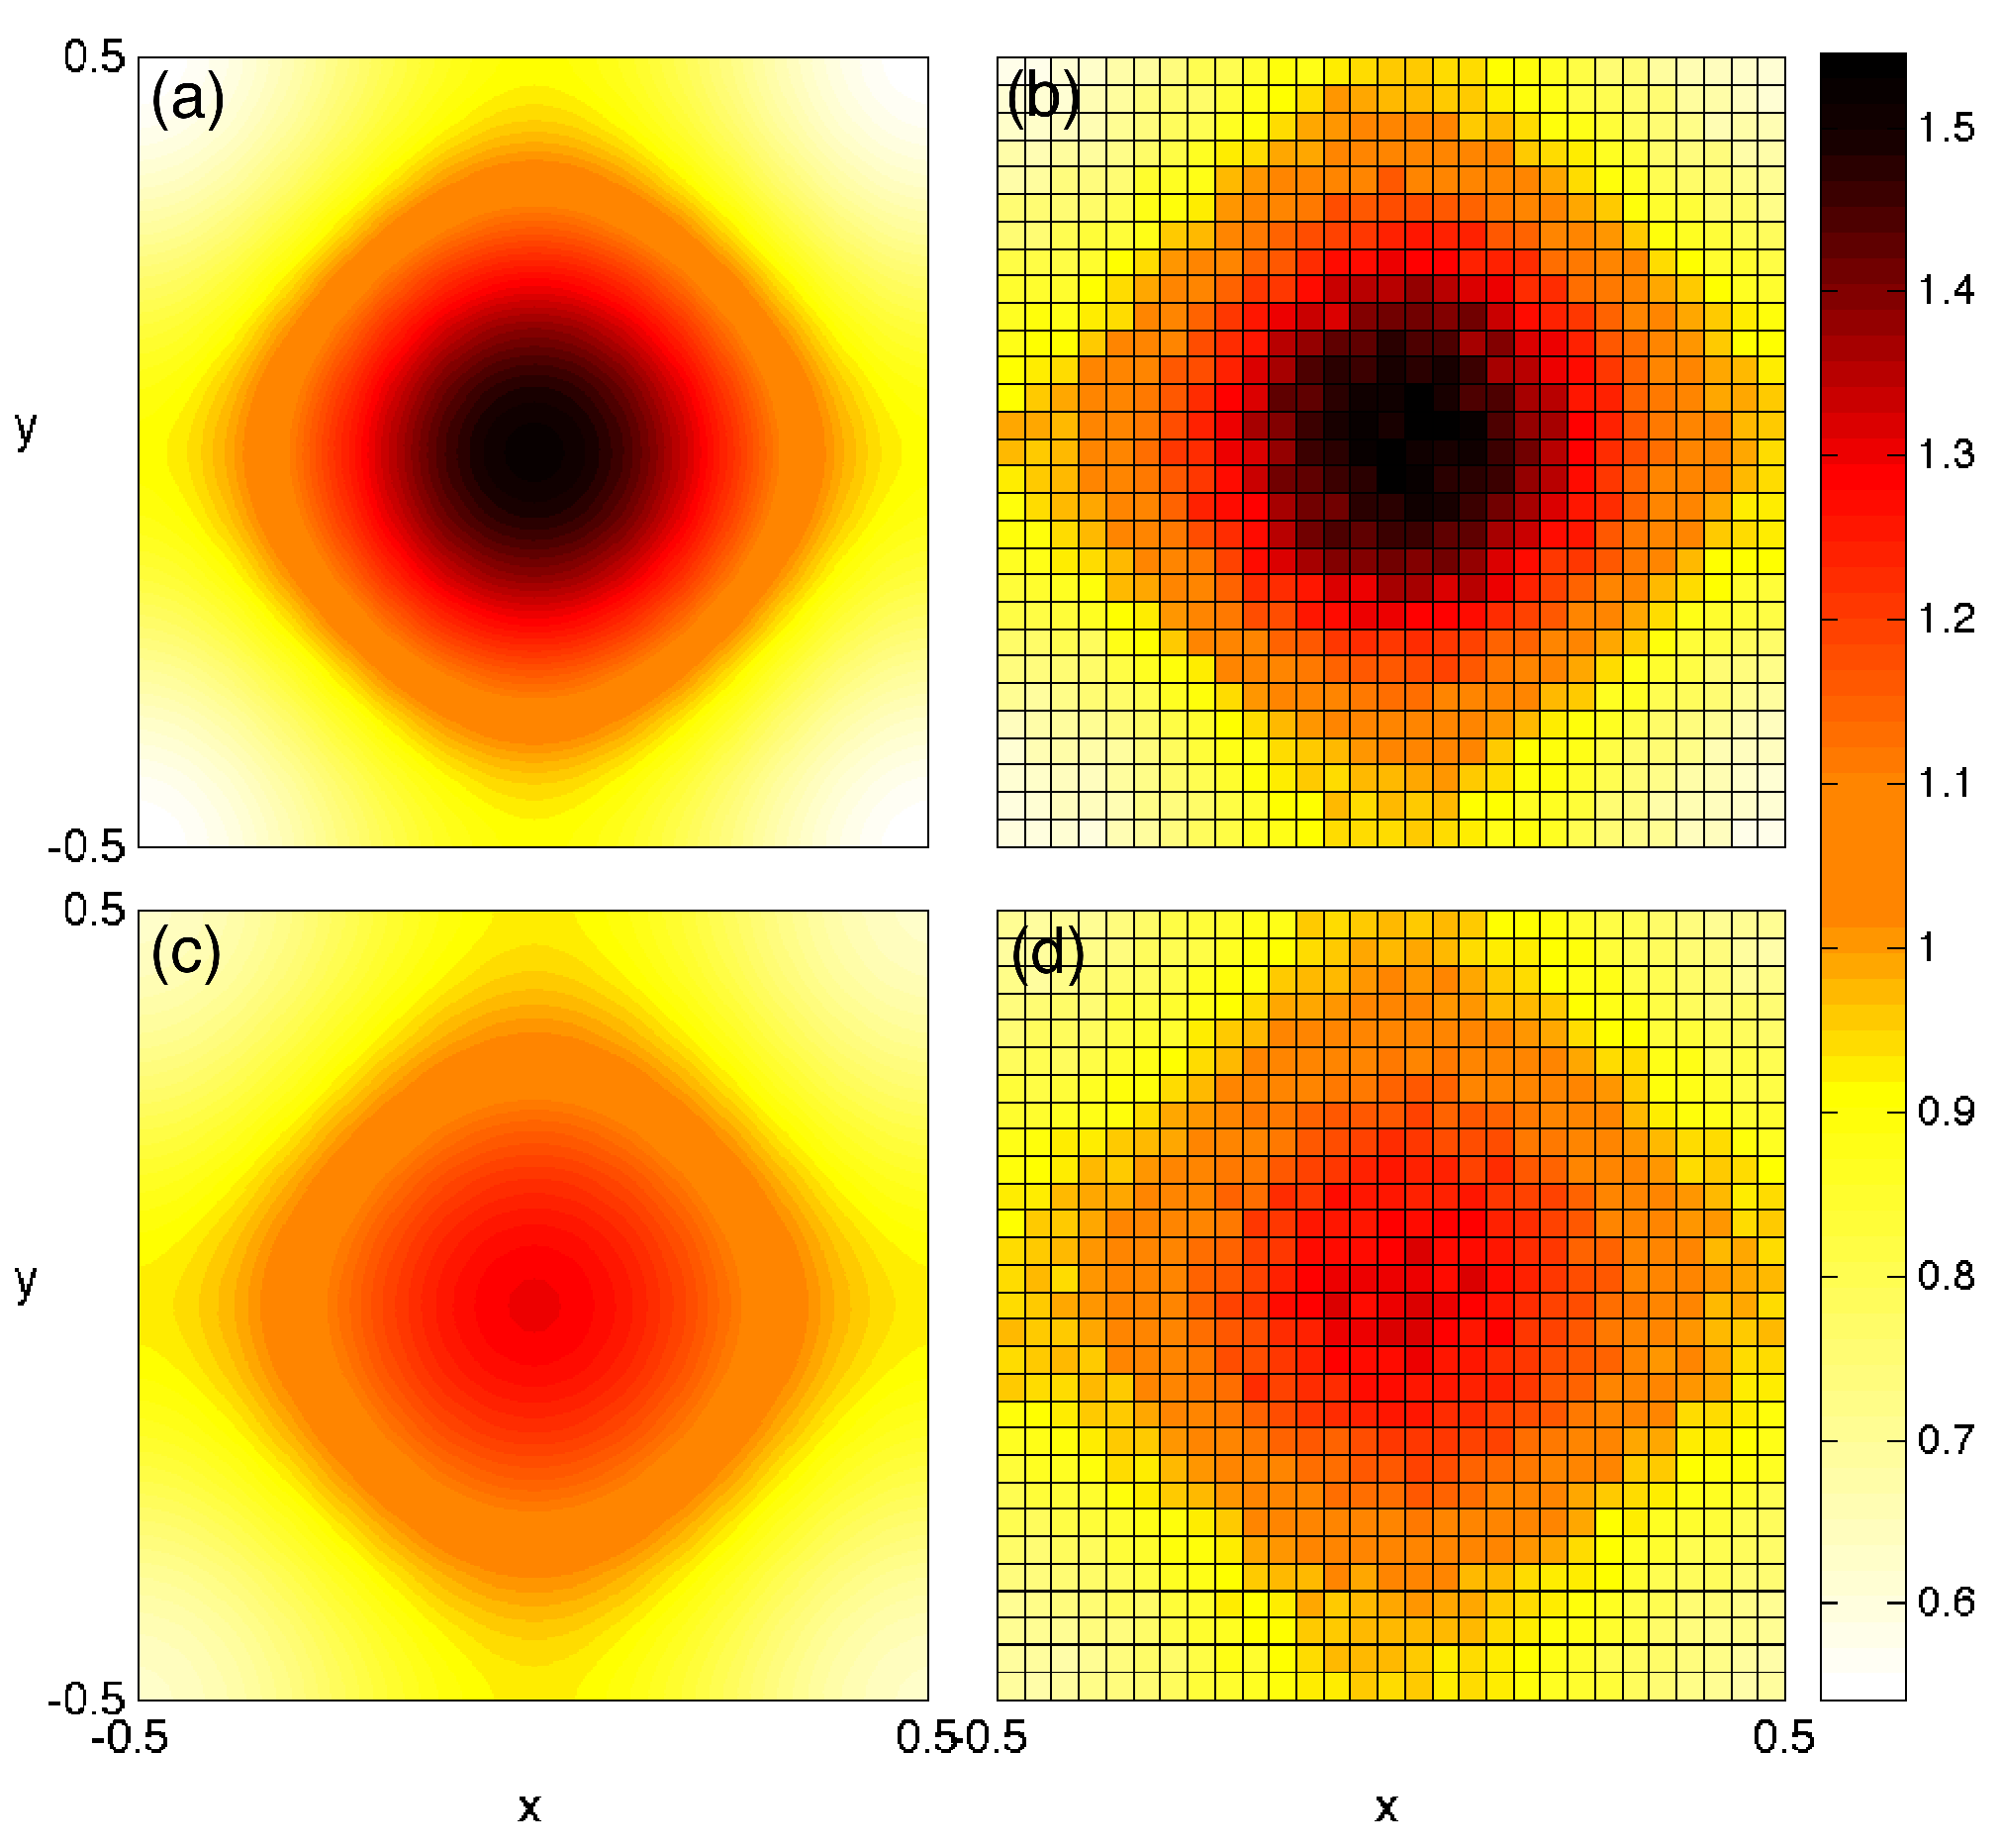
\includegraphics[width=\textwidth*2/3]{sanity-check/fig2_BC12.png}
    \caption{
    This figure contains the following four plots, all of them are shown at time \( t=0.05 \): \newline
    \hspace*{0.5em}(a) shows the solution of the linear diffusion equation~\ref{eq:heat} for point particles. \newline
    \hspace*{0.5em}(b) shows the histogram of a Monte Carlo simulation of the point particle model. \newline
    \hspace*{0.5em}(c) shows the solution of the nonlinear diffusion equation~\ref{eq:hard-sphere-p} for finite-sized particles. \newline
    \hspace*{0.5em}(d) shows the histogram of a Monte Carlo simulation of the HSCM. \newline
    For the two lower plots (c) and (d), a higher diffusion rate can be observed. 
    The Monte Carlo simulations used $10^4$ simulation runs each with a time step size of $10^-5$.
    }
    \label{fig:fig2BC12}
\end{figure}

\subsection{Reproduction of reference results}
Before running our new dynamics that include cell flexibility, we first want to guarantee that the simulations are running in the correct setup.
Therefore, we started with recreating the Monte Carlo simulation for the point particles. 
I always fixed the color scale to be the same as in~\cite{Bruna2012} in order to gain comparability. 
The simulation parameters are the same as in~\cite{Bruna2012}. \\
All of our simulations run in the Julia programming language. 
There, we used the package `DifferentialEquations.jl' with its structure `SDEProblem()' and then solved it with the package inbuilt Euler Maruyama scheme that uses a constant time step size. \\
I employed a callback function that was triggered after each simulation step to implement a reflective boundary condition. 
Whenever a particle moved outside the domain, it was relocated to the position within the domain such that its distance to the domain boundary remained unchanged, effectively reflecting the particle off the boundary. \\
Beside of this, all particles moved according to the two dimensional Brownian motion
\begin{center}
		$ \dequ \vec{x}_i(t) = \sqrt{2} \dequ \vec{B}^{\:i}$, \hspace{0.5em} $1 \leq i \leq N_{C}$.
\end{center}
Figure~\ref{fig:ppHeatmaps} shows the evolution of the particle density in terms of heatmaps for different time steps. 
The results of our Monte Carlo simulation appear to be in good agreement with those of Bruna and Chapman, suggesting that our approach is robust and accurate.

Next, we consider the HSCM and run the Monte Carlo simulation for a cell diameter of $\epsilon = 0.01$. 
Figure~\ref{fig:hscmHeatmaps} shows the density evolution of the HSCM.
%%% TODO: tell that we want to test what our model delivers 
%%% TODO: conclude that we hopefully have matching results 

\begin{figure}[h]
	\centering
    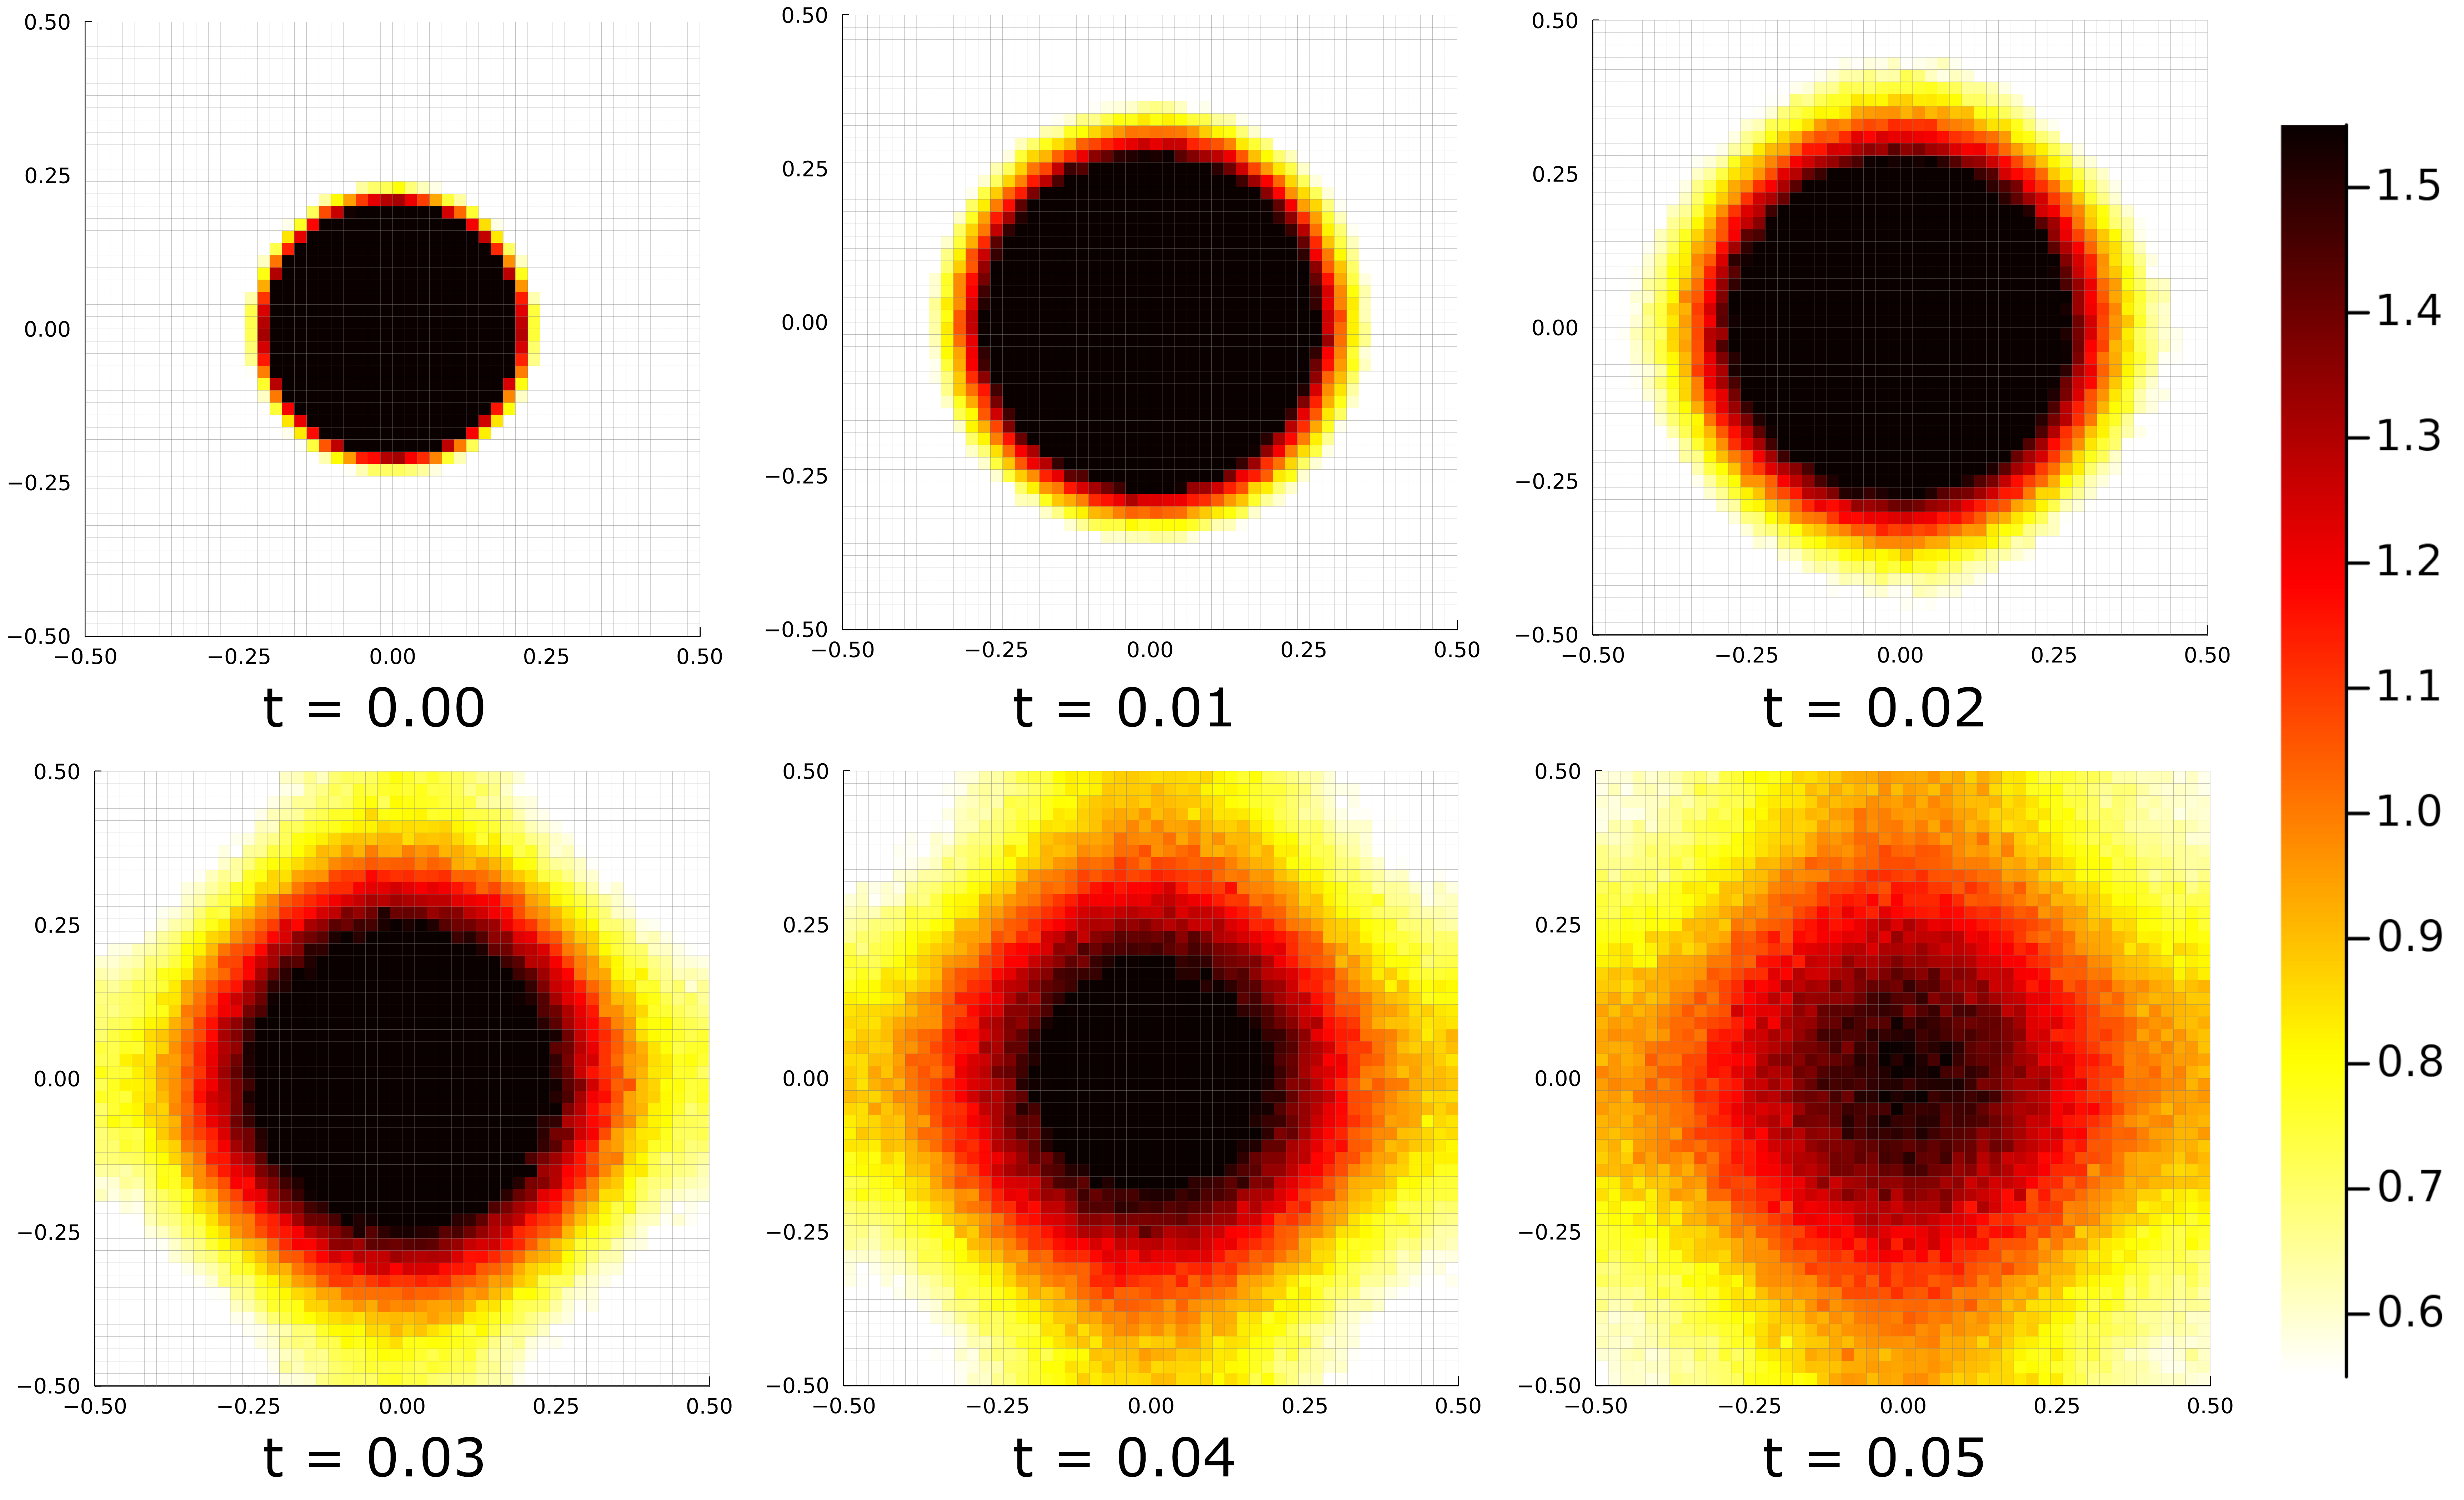
\includegraphics[width=\textwidth]{sanity-check/ppHeatmaps_50x50.png}
    \caption{Heatmaps of a Monte Carlo simulation of the point particle model at the times $t \in \{0.00, 0.01, 0.02, 0.03, 0.04, 0.05\}$. 
    They visualise the evolution of the particle density over time. 
    ppHeatmaps$50$. 
    }
    \label{fig:ppHeatmaps}
\end{figure}

\begin{figure}[h]
	\centering
    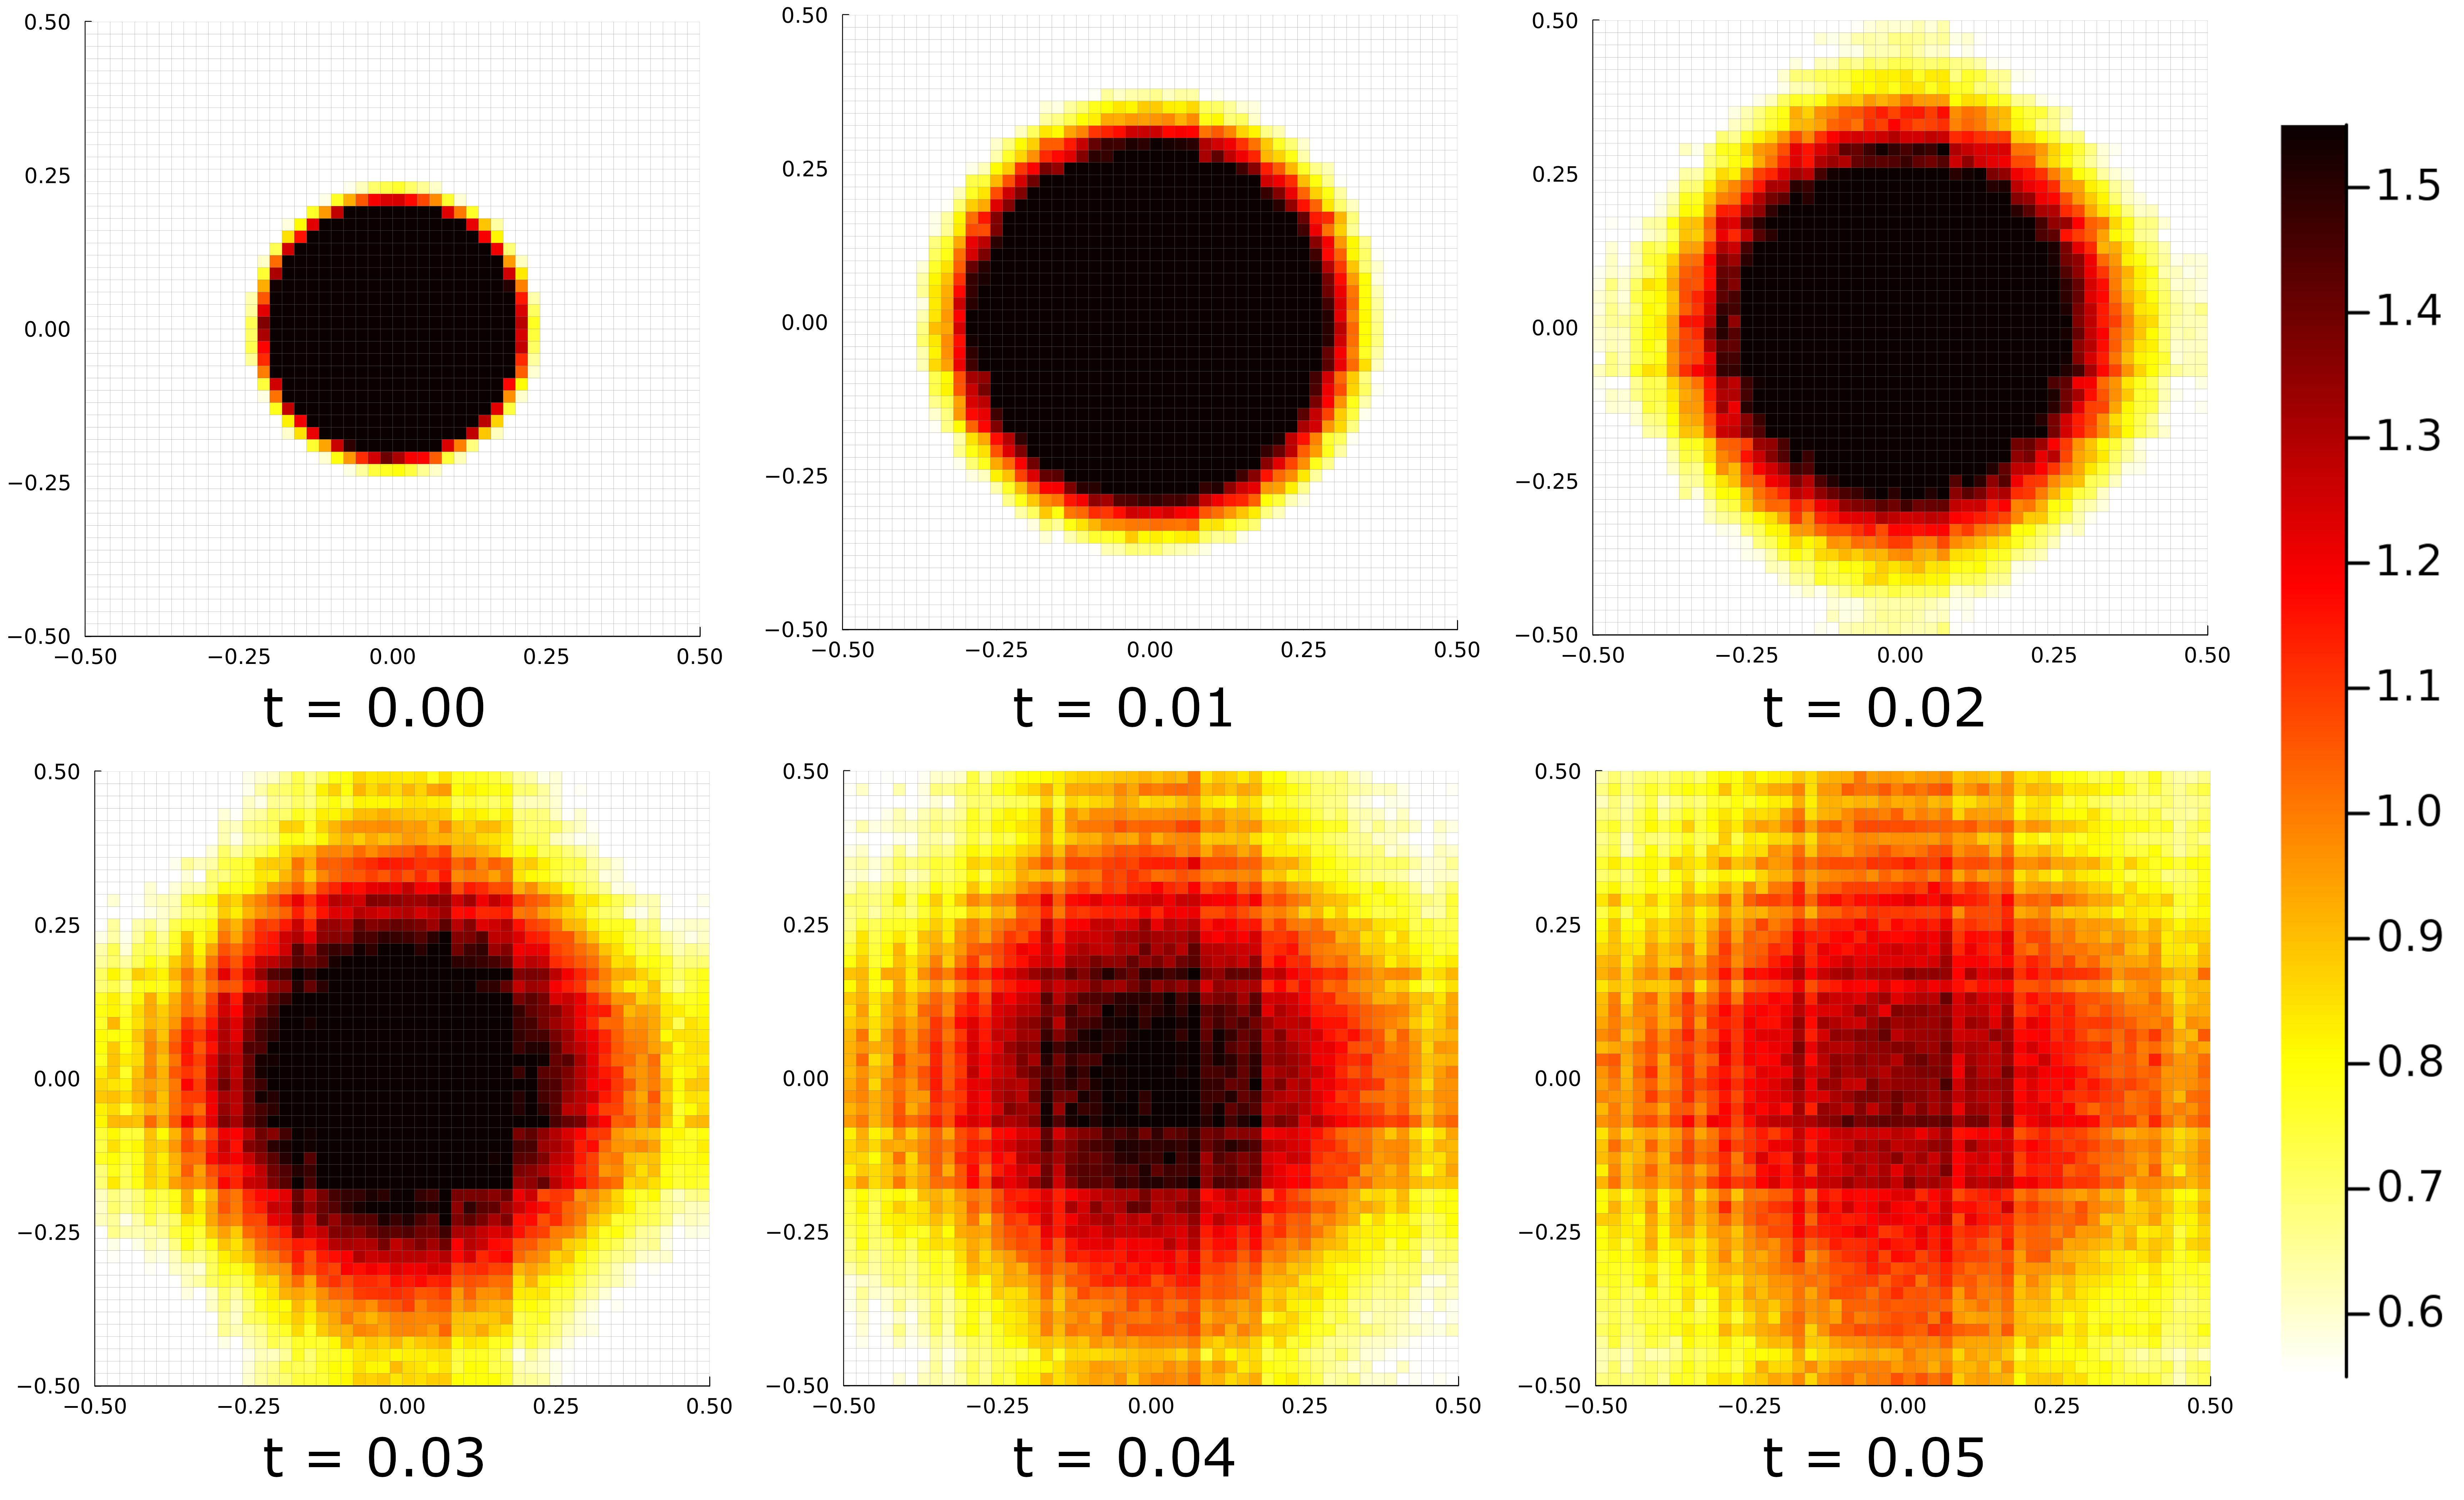
\includegraphics[width=\textwidth]{sanity-check/hscmHeatmaps_callback_50x50.png}
    \caption{Heatmaps of a Monte Carlo simulation of the hard sphere cell model at the times $t \in \{0.00, 0.01, 0.02, 0.03, 0.04, 0.05\}$. 
    They visualise the evolution of the particle density over time. 
    hscmHeatmapscallback$50$.
    }
    \label{fig:hscmHeatmaps}
\end{figure}


\begin{figure}[h]
	\centering
    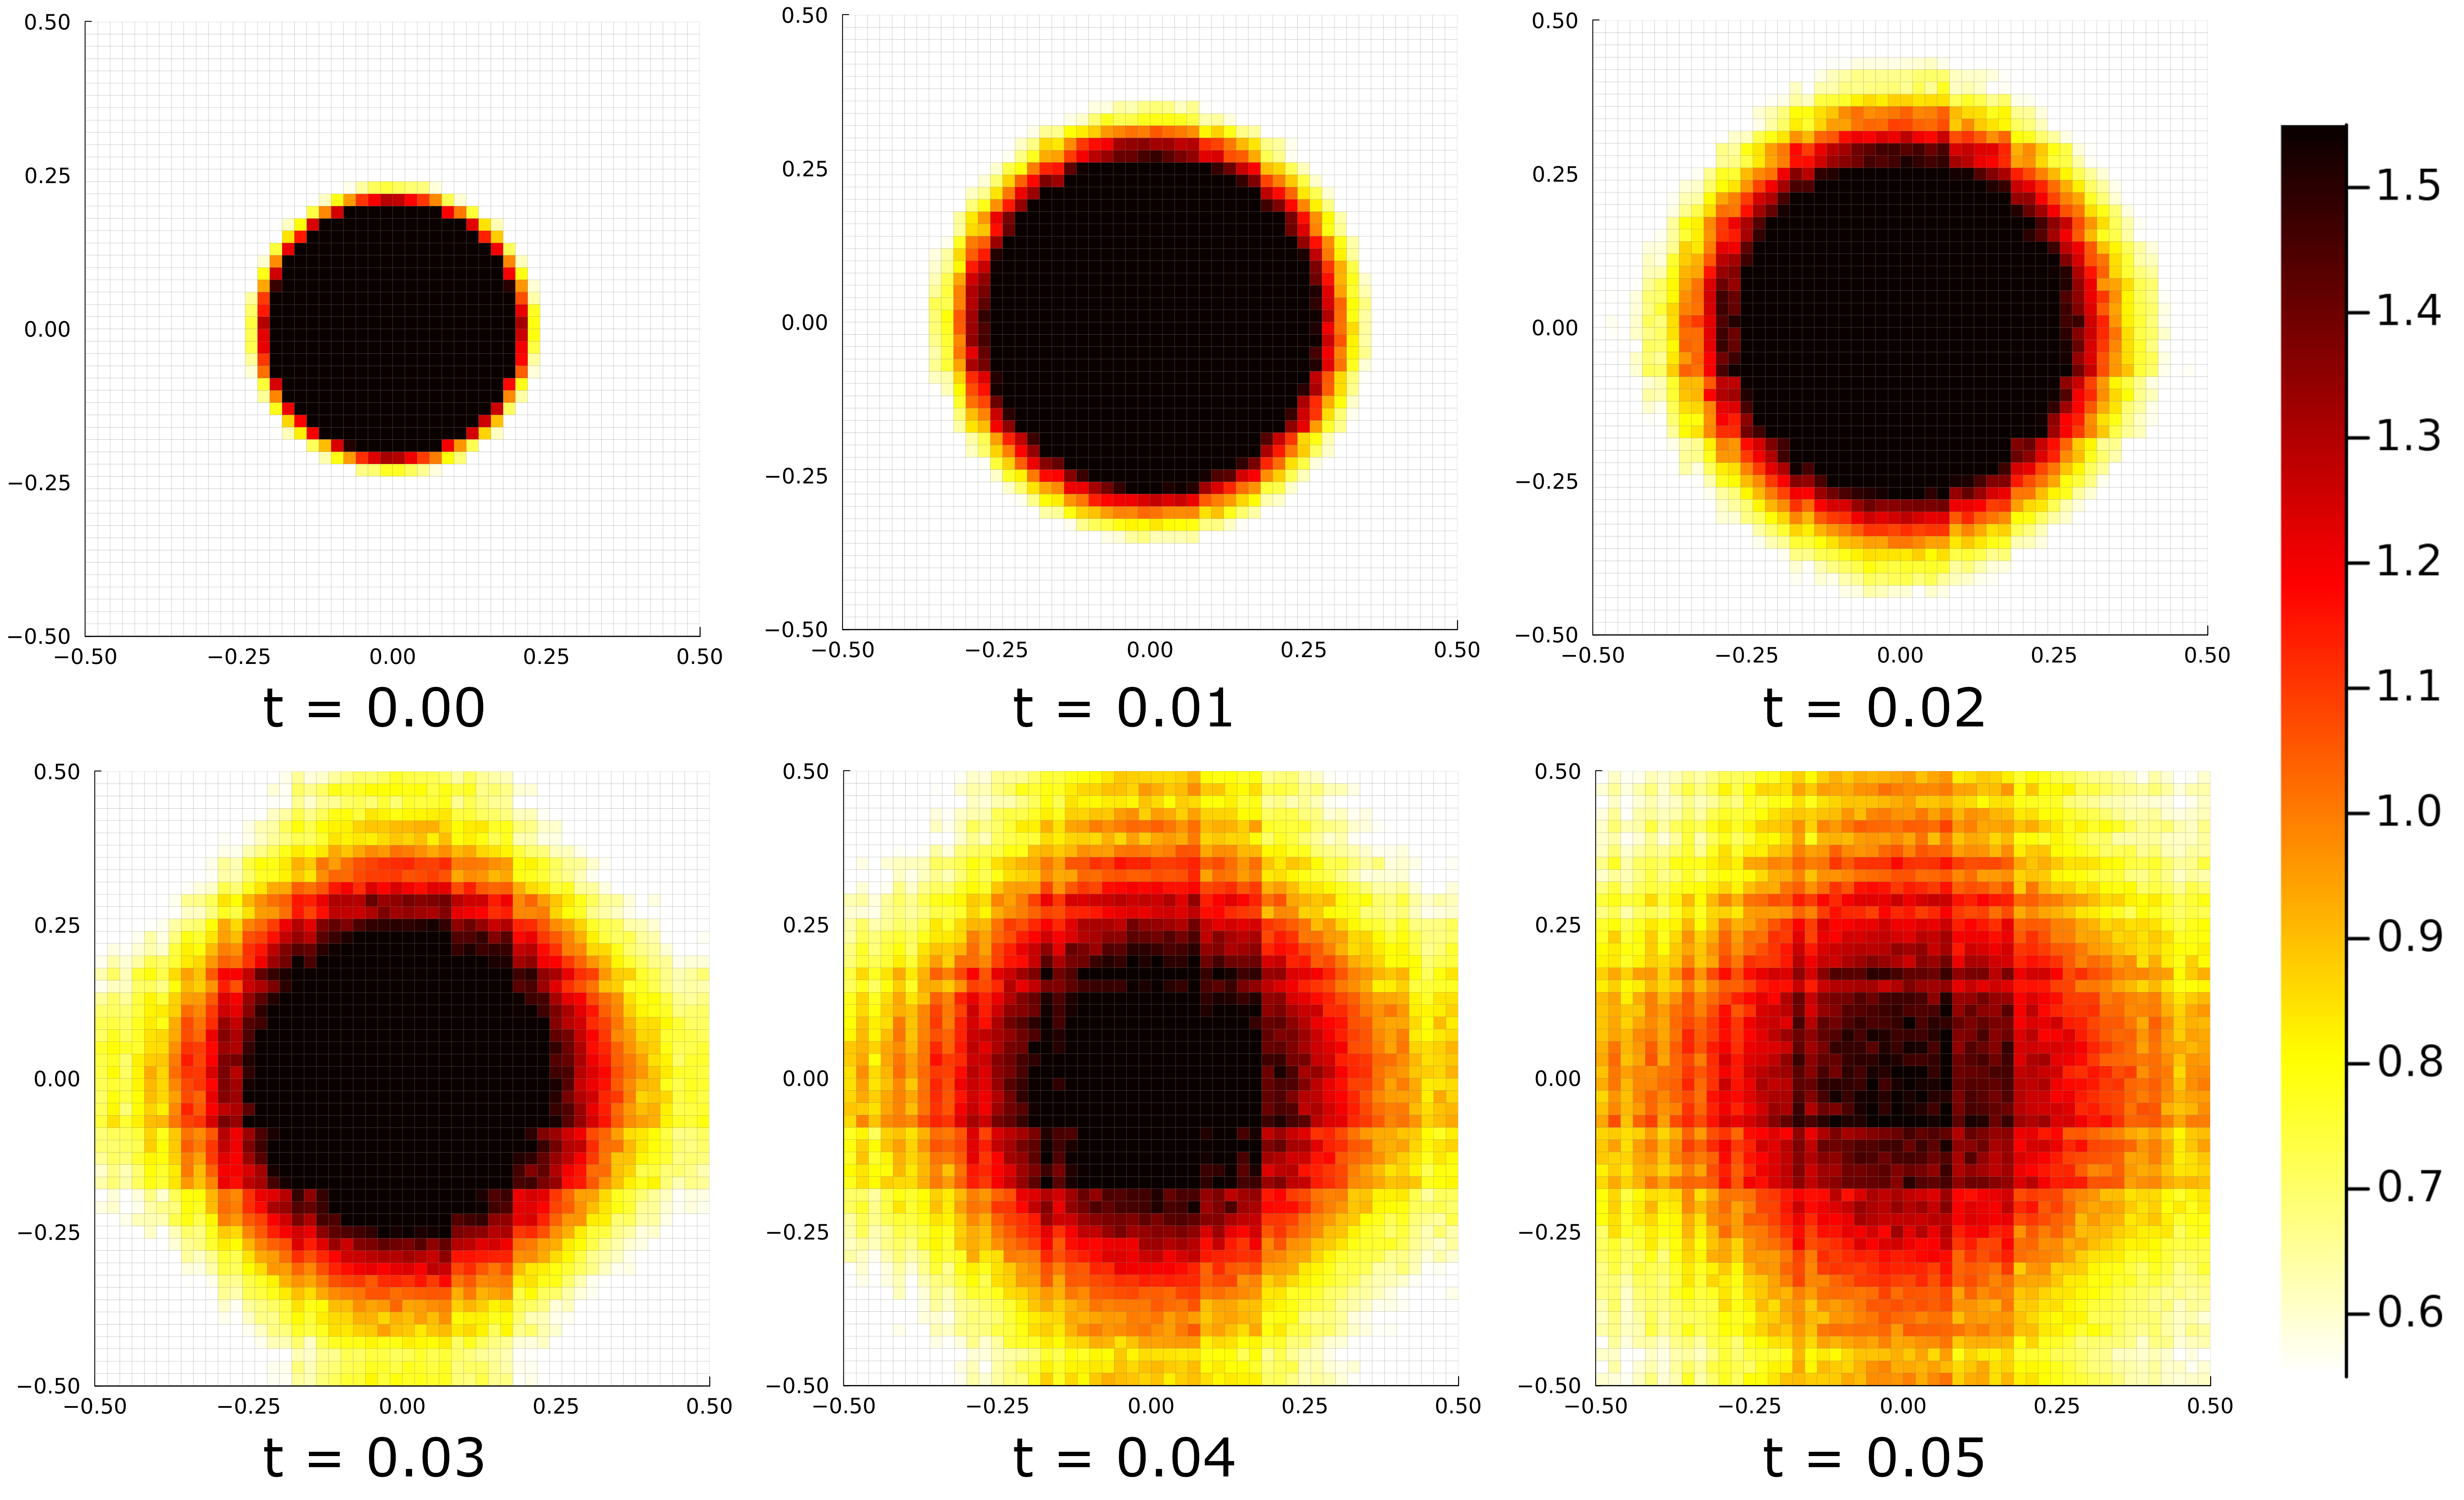
\includegraphics[width=\textwidth]{sanity-check/hscmHeatmaps_billard_50x50.png}
    \caption{Heatmaps of a Monte Carlo simulation of the point particle model at the times $t \in \{0.00, 0.01, 0.02, 0.03, 0.04, 0.05\}$. 
    They visualise the evolution of the particle density over time. 
    hscmHeatmapsbillard$50$.
    }
    \label{fig:ppHeatmaps}
\end{figure}




\begin{figure}[h]
	\centering
    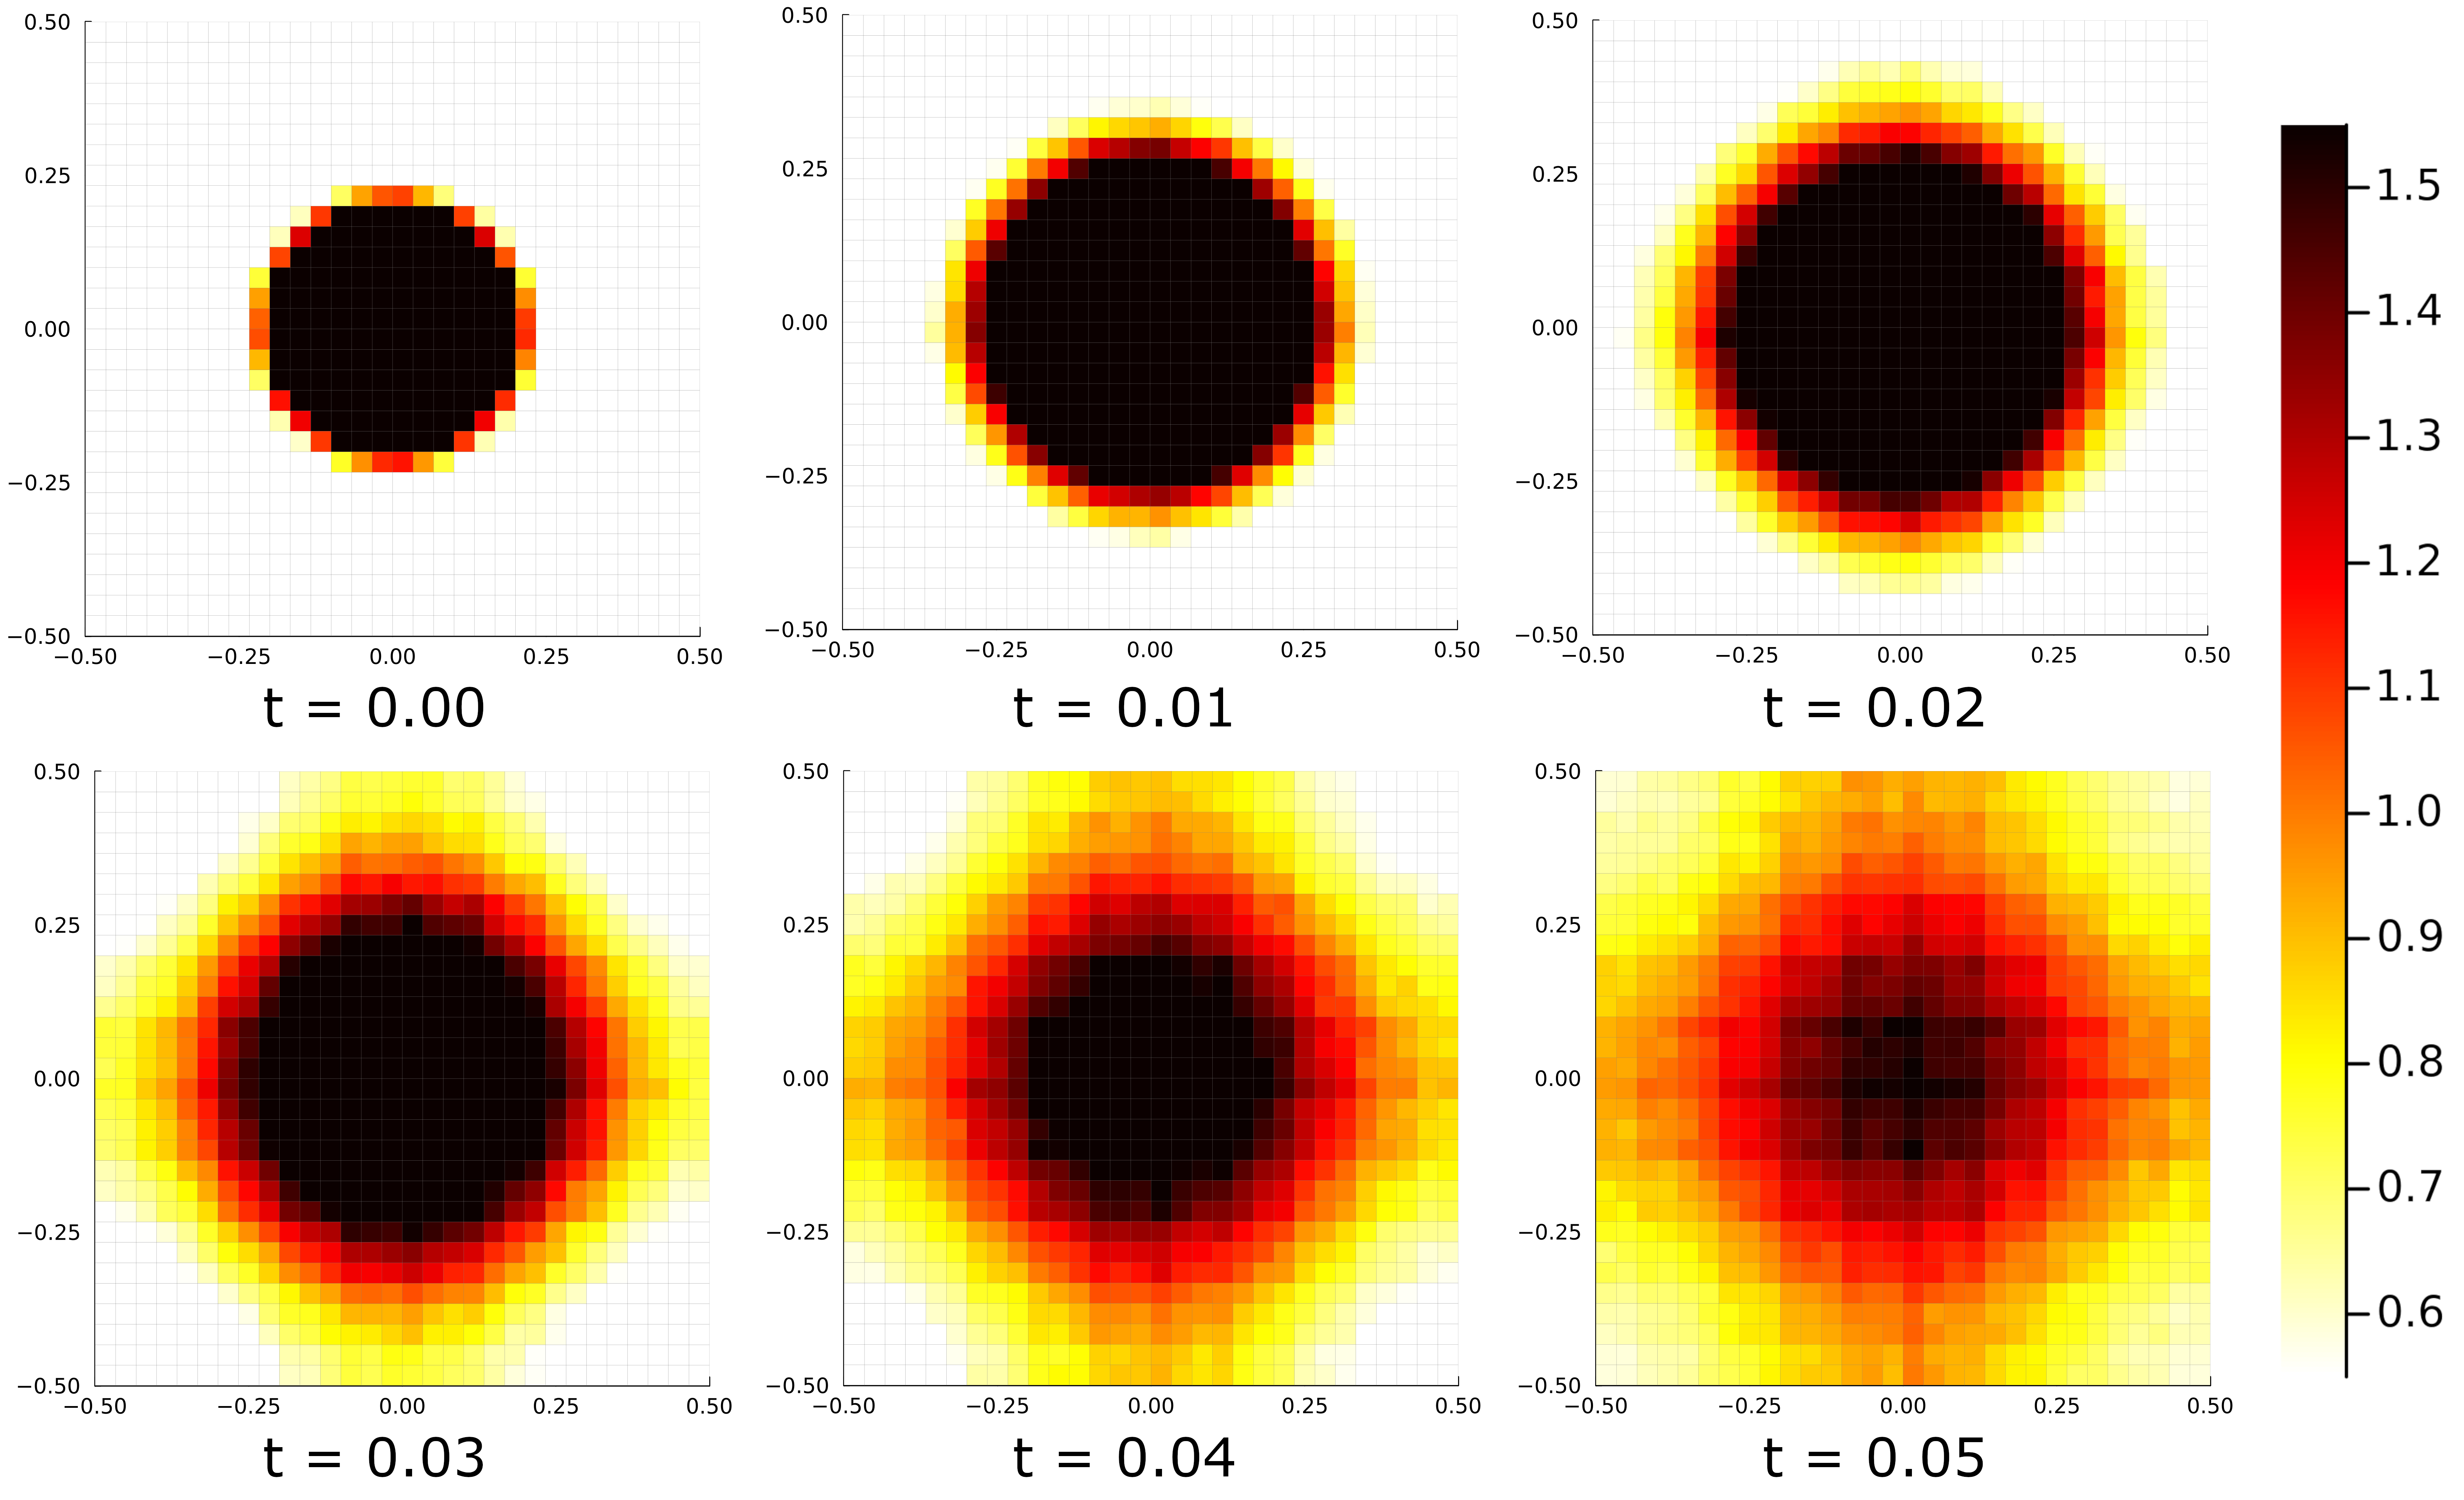
\includegraphics[width=\textwidth]{sanity-check/ppHeatmaps_30x30.png}
    \caption{Heatmaps of a Monte Carlo simulation of the point particle model at the times $t \in \{0.00, 0.01, 0.02, 0.03, 0.04, 0.05\}$. 
    They visualise the evolution of the particle density over time. 
    ppHeatmaps$30$. 
    }
    \label{fig:ppHeatmaps}
\end{figure}

\begin{figure}[h]
	\centering
    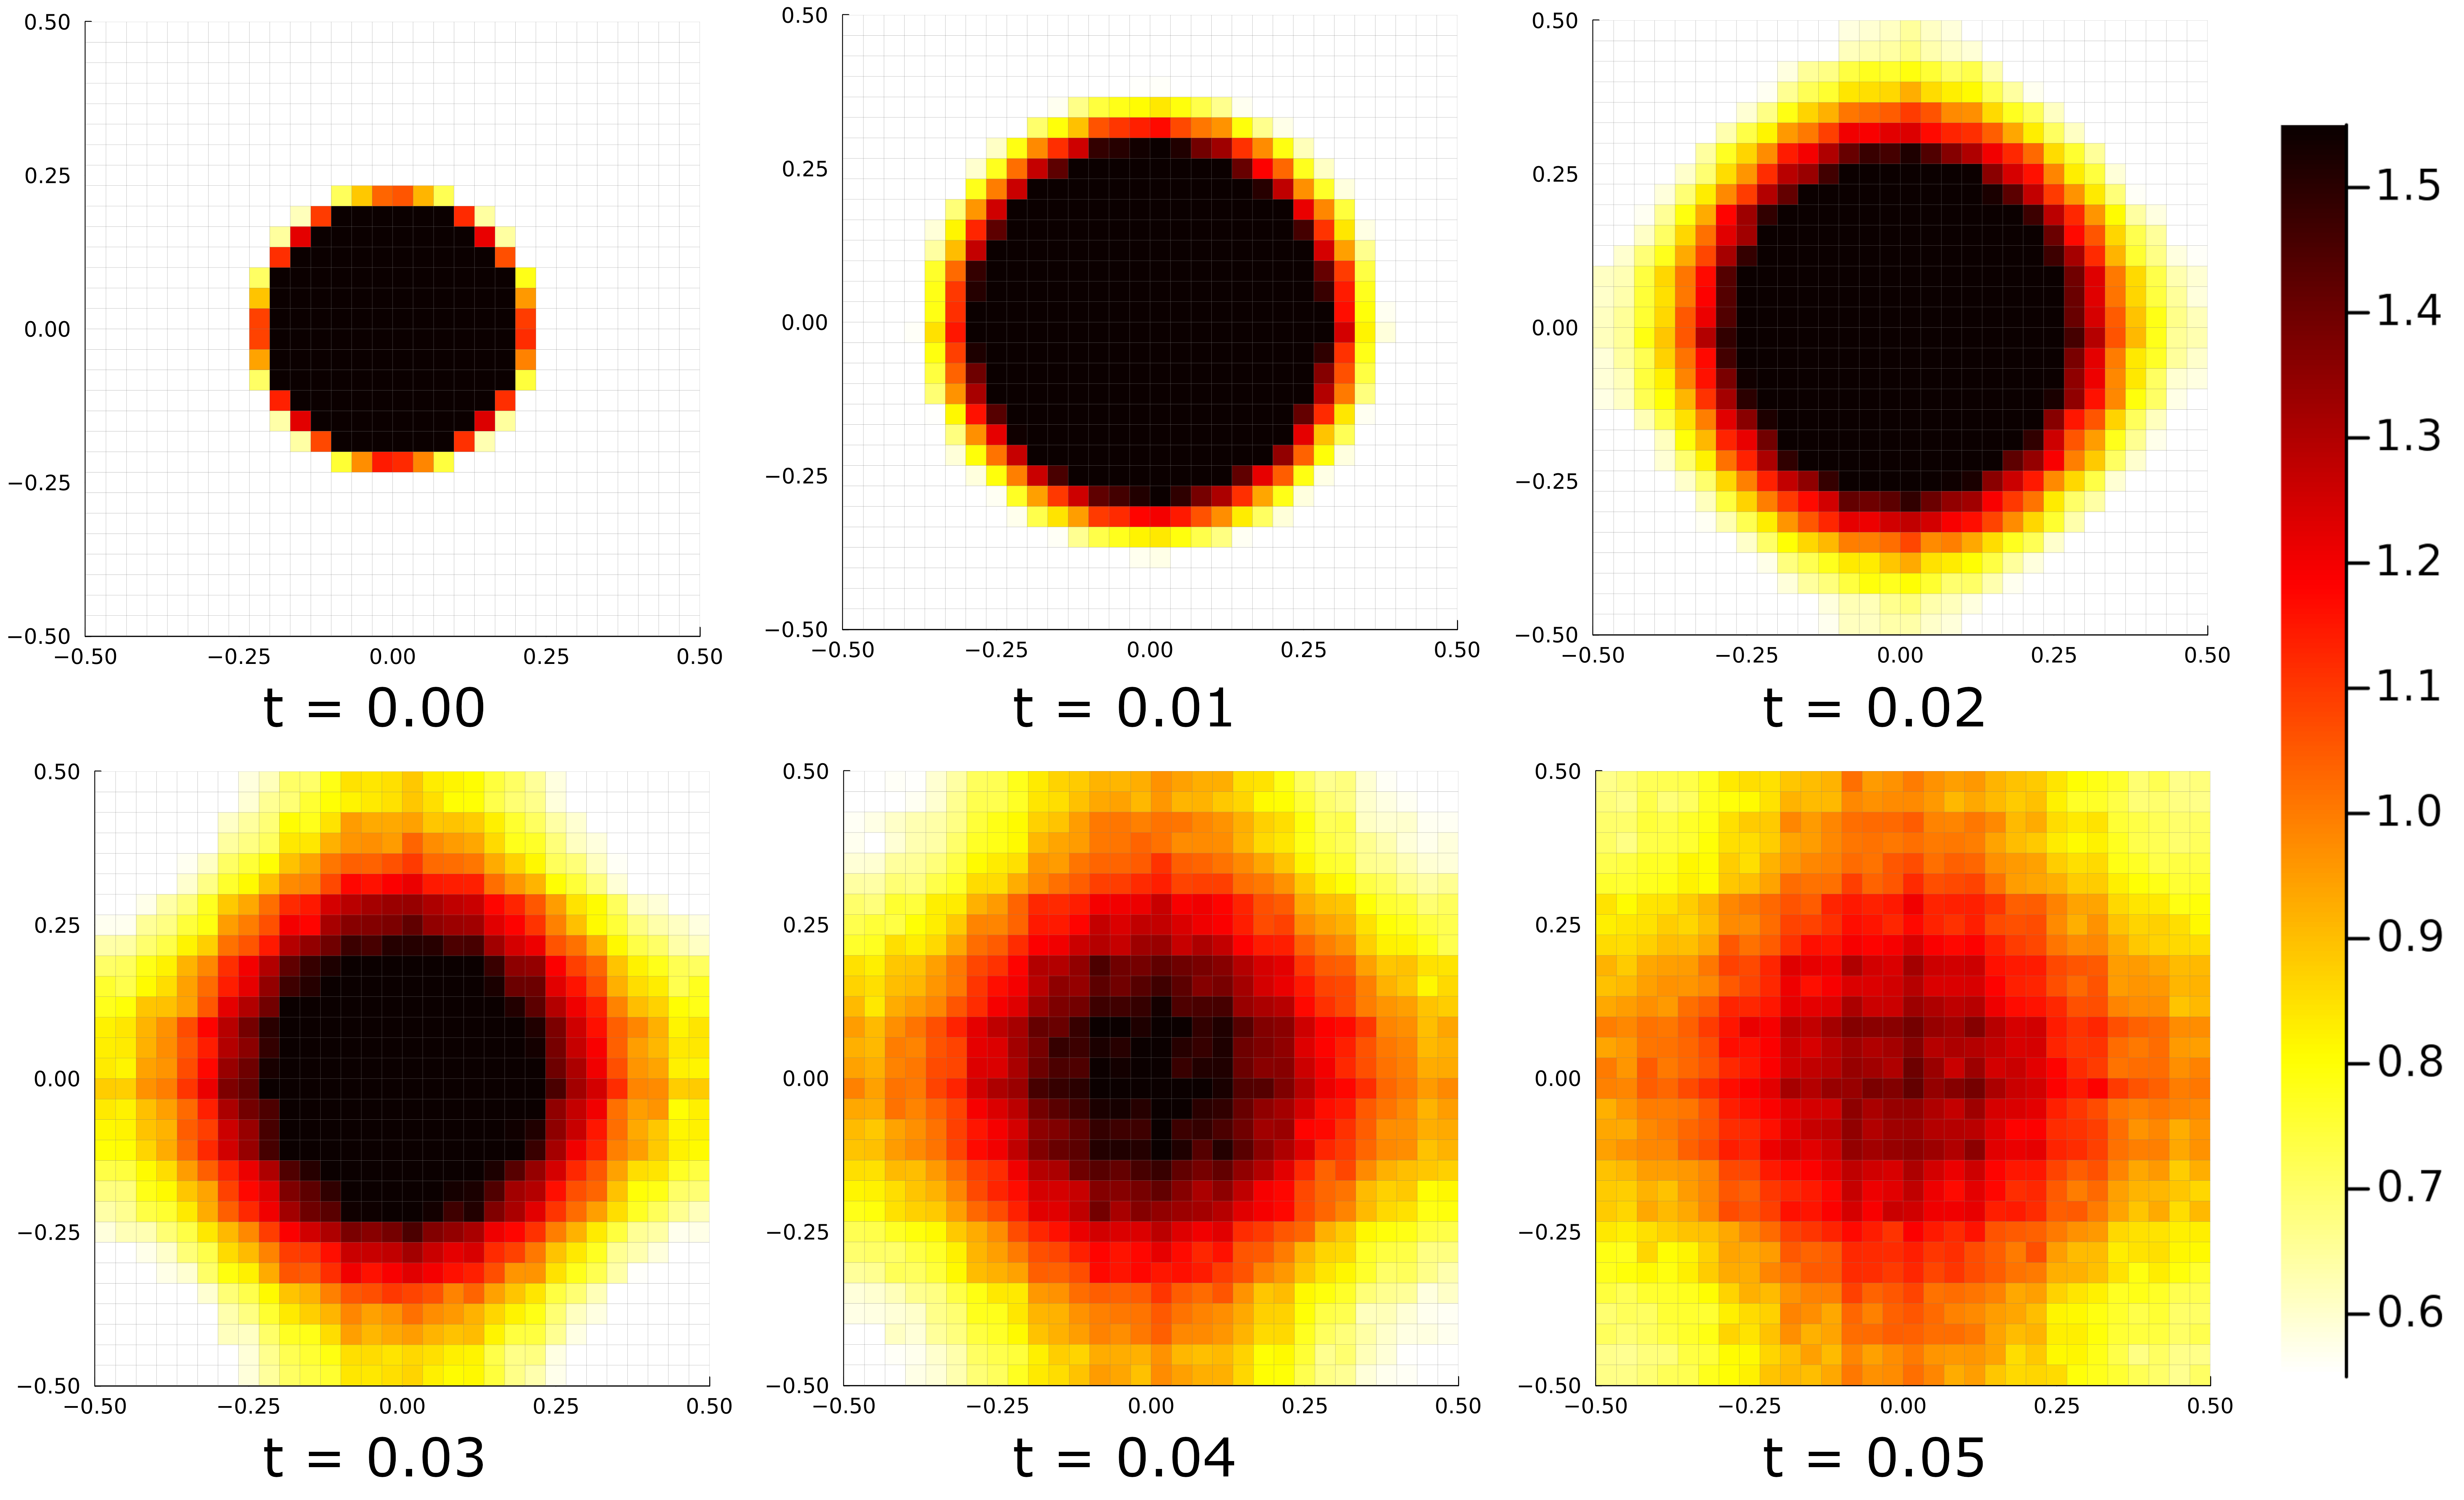
\includegraphics[width=\textwidth]{sanity-check/hscmHeatmaps_callback_30x30.png}
    \caption{Heatmaps of a Monte Carlo simulation of the hard sphere cell model at the times $t \in \{0.00, 0.01, 0.02, 0.03, 0.04, 0.05\}$. 
    They visualise the evolution of the particle density over time. 
    hscmHeatmapscallback$30$.
    }
    \label{fig:hscmHeatmaps}
\end{figure}


\begin{figure}[h]
	\centering
    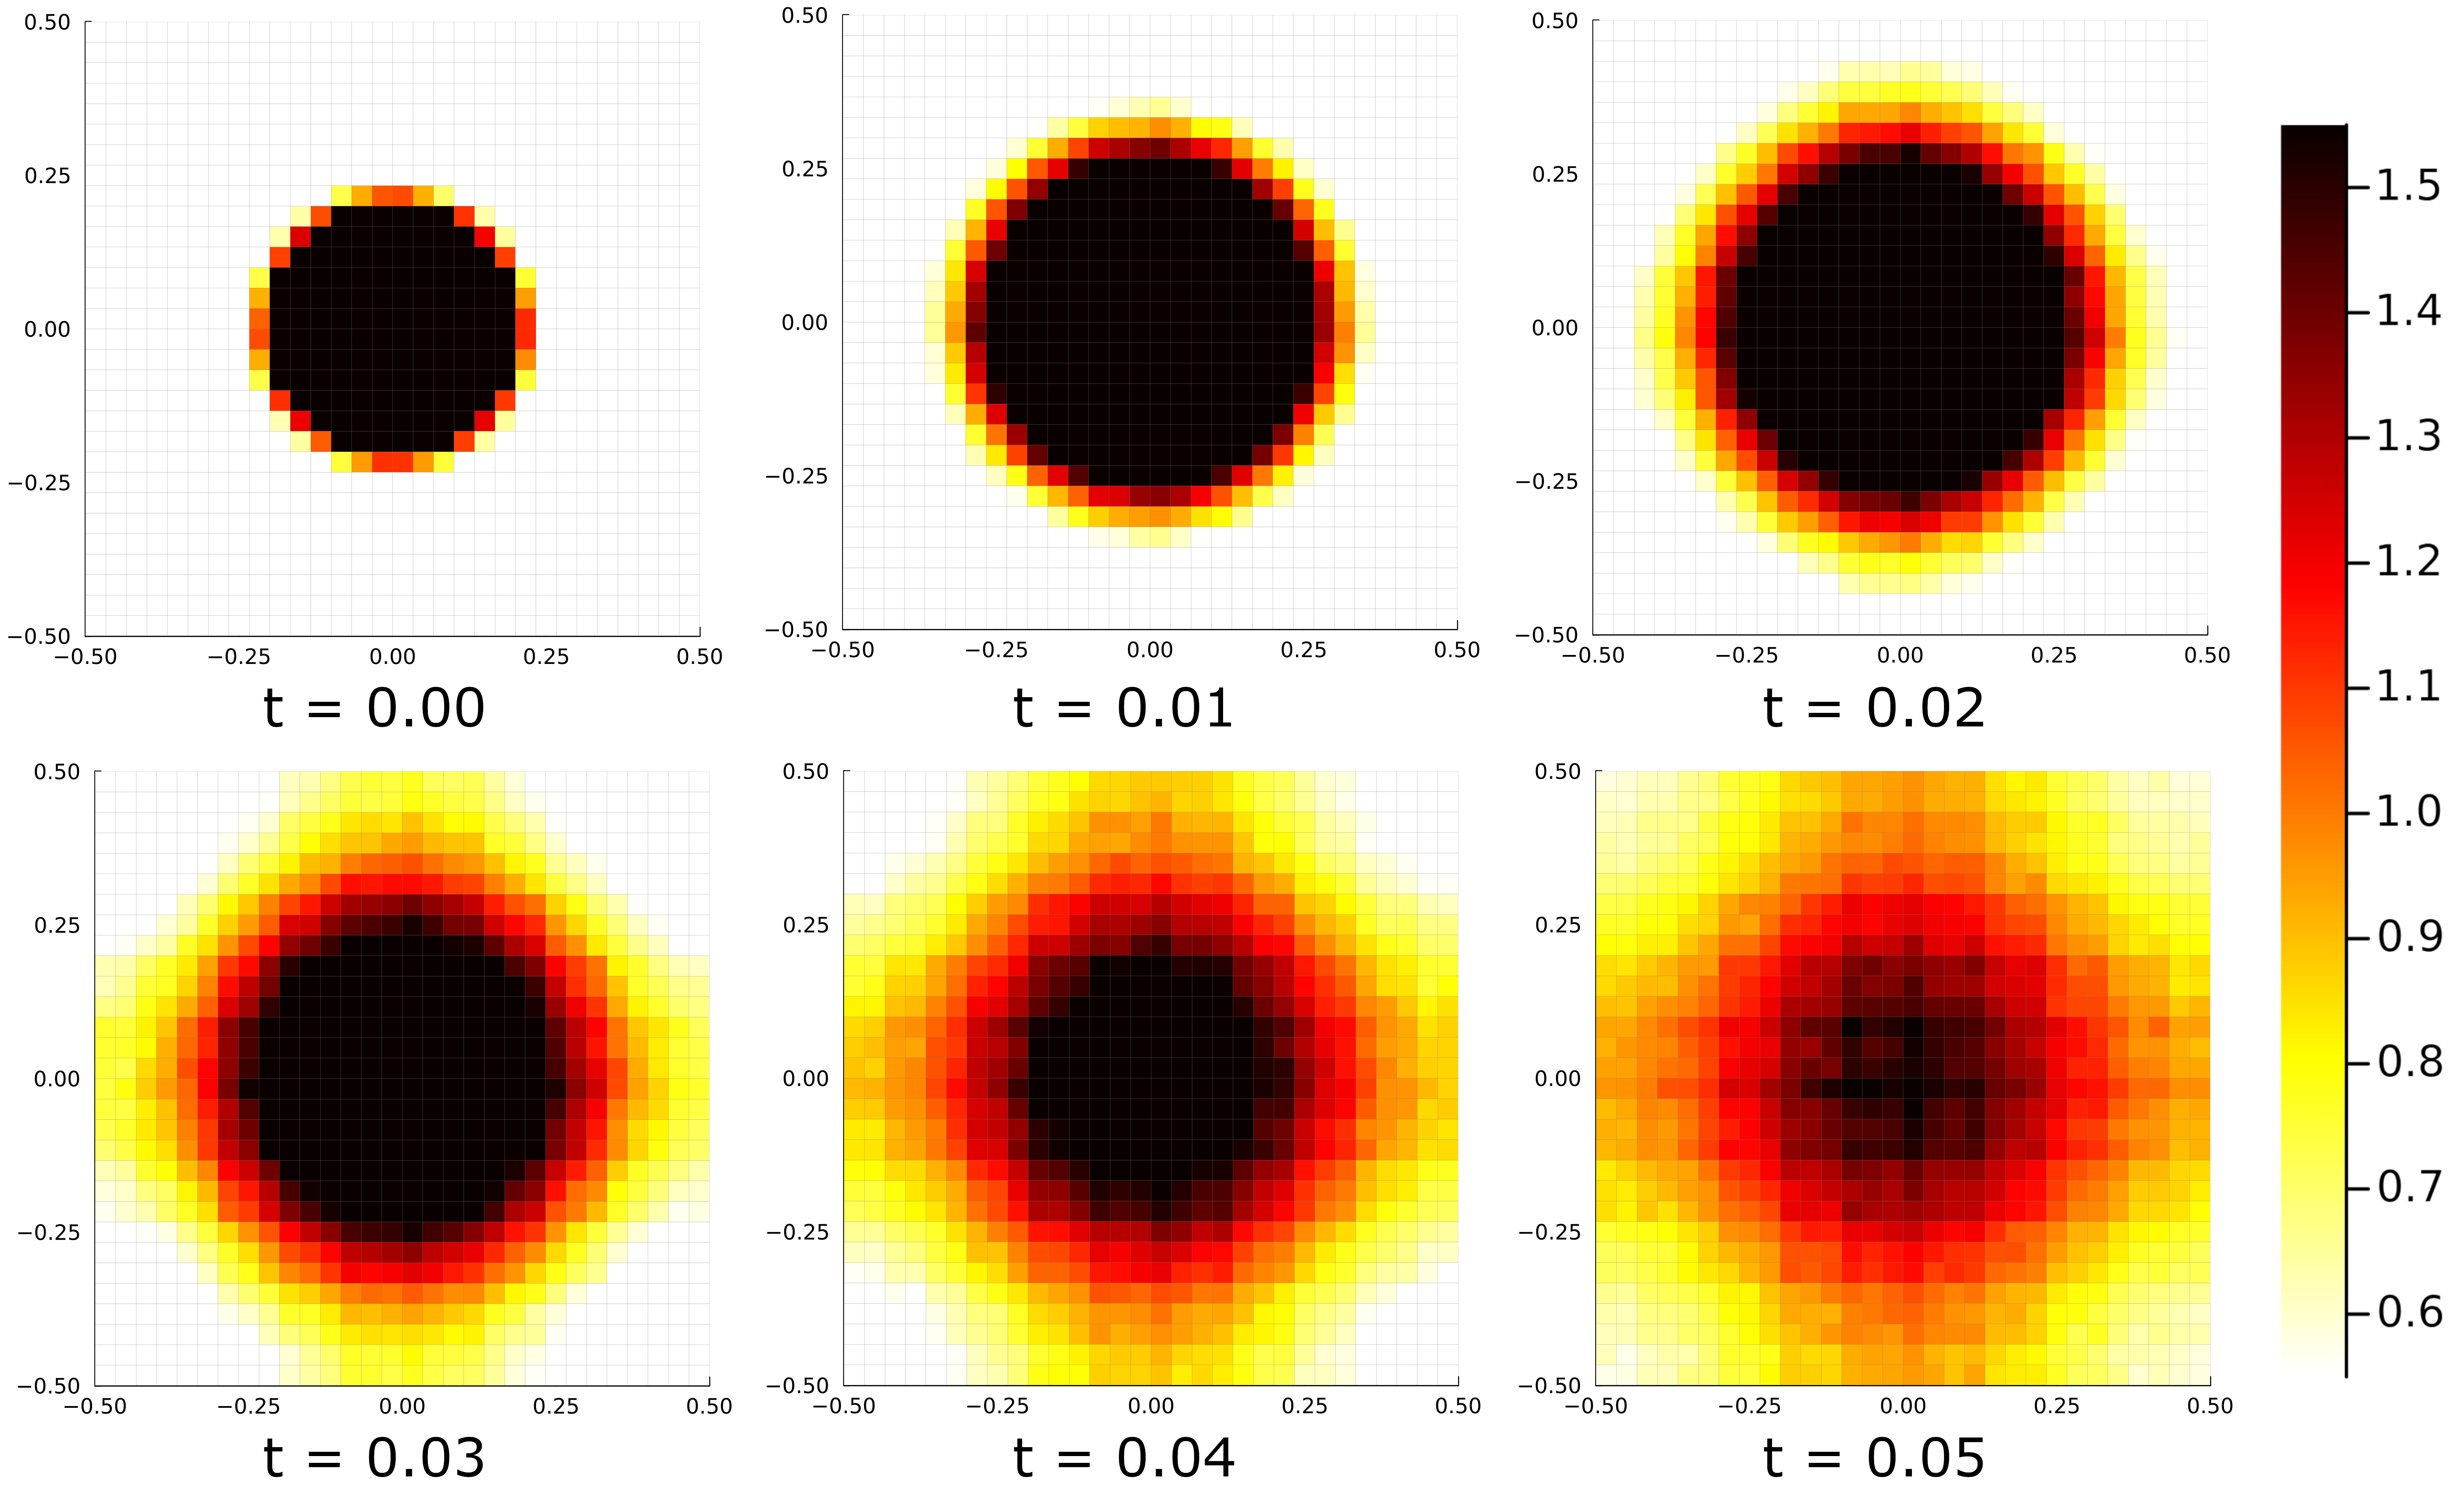
\includegraphics[width=\textwidth]{sanity-check/hscmHeatmaps_billard_30x30.png}
    \caption{Heatmaps of a Monte Carlo simulation of the point particle model at the times $t \in \{0.00, 0.01, 0.02, 0.03, 0.04, 0.05\}$. 
    They visualise the evolution of the particle density over time. 
    hscmHeatmapsbillard$30$.
    }
    \label{fig:ppHeatmaps}
\end{figure}